\begin{frame}		
	\frametitle{Task 1}
	\framesubtitle{Echo Server}
	
	\begin{figure}[H]
		\center{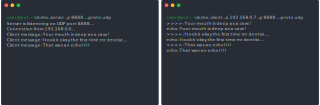
\includegraphics[width = 1\textwidth]{echo-example}}
	\end{figure}
	
	\footnotetext{Demo: \href{https://www2.tkn.tu-berlin.de/teaching/rn/animations/}{1}, \href{https://wps.pearsoned.com/ecs_kurose_compnetw_6/216/55463/14198702.cw/index.html}{2}}
\end{frame}

\begin{frame}[fragile]
	\frametitle{Task 2}
	\framesubtitle{Network condition simulation}
	
Your task is to create Python program which transmits files via network under harsh network conditions.

	
\end{frame}



\begin{frame}[fragile]
	\frametitle{Task 2}
	\framesubtitle{Network condition simulation}

Filesize: 1 GB
Bandwidth: 100 Mbps
MTU: 1512 B	
	
\begin{table}
	\begin{tabular}{ | r | r | c | c | c | c | c | }
		RTT, msec & PLR     & 4 credits & 8 credits   & 11 credits     & 15  credits   \\ \hline \hline
		1         & 0 \%    & 25 min & 20 min & 15 min & 10 min \\ 
		10        & 1 \%    & 30 min & 25 min & 20 min & 15 min \\
		10        & 10 \%   &        & 30 min & 25 min & 20 min \\
		100       & 10 \%   &        &        & 30 min & 25 min \\
		1000      & 1  \%   &        &        &        & 30 min  
	\end{tabular}
	\caption{Cases and credits}
\end{table}

Stop-and-Wait gets 4 credits. Go-Back-N gets 8 credits. Selective repeate gets 11 credits.

\end{frame}


\begin{frame}[fragile]
	\frametitle{Task 2}
	\framesubtitle{Network condition simulation}
	
	
	\begin{semiverbatim}
		# to set delays and losses on eth0 interface
		tc qdisc add dev eth0 root netem delay 10ms loss 1.0%
		# to remove delays and losses on eth0 interface
		tc qdisc del dev eth0 root netem delay 10ms loss 1.0%
		# to limit bandwith on eth0 interface
		tc qdisc add dev eth0 root tbf rate 100mbit
		# to check network parammeters
		iperf3 -s -p 8888 # server side
		iperf3 -c 127.0.0.1 -p 8888 -u -b 1000m # client side
	\end{semiverbatim}


	\footnotetext{\href{https://www.techrepublic.com/article/how-to-limit-bandwidth-on-linux-to-better-test-your-applications/}{How to limit bandwidth on \\Linux to better test your applications} }

\end{frame}


\begin{frame}[fragile]
	\frametitle{Task 2}
	\framesubtitle{How it should look like}
	
	\begin{figure}[H]
		\center{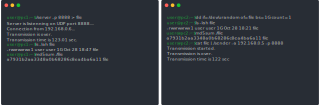
\includegraphics[width = 1\textwidth]{transmission-example}}
	\end{figure}
	
\end{frame}

